\documentclass[letterpaper, 12pt]{article}
\usepackage[american]{babel}
\usepackage[utf8]{inputenc}
\usepackage[citestyle=apa,style=apa,backend=biber]{biblatex}
\usepackage[margin=1in]{geometry}
\usepackage{graphicx}
\usepackage{caption}
\usepackage{float}
\setlength\bibitemsep{2\itemsep}
\DeclareLanguageMapping{american}{american-apa}
\addbibresource{bibliography.bib}

\pagenumbering{roman}

\begin{document}
\begin{titlepage}
\centering
	\vspace*{5.75cm}
	{\huge\bfseries A literature review of Internet of Things security\par}
	\vspace{2cm}
	Blair Urish\\
	Kansas State University\\
	College of Engineering\\
	Department of Computer Science\\
	\vspace{1cm}
	Dr. William Hsu\\
	Professor\\
	Department of Computer Science\\
	\vspace{1cm}
	May 4 2017
\end{titlepage}


\begin{abstract}
\thispagestyle{plain}
\setcounter{page}{2}
\begin{flushleft}
	The Internet of Things (IoT) is a rapidly growing industry with lots of potential for innovation. By 2020, it is expected that
there will be 25 million IoT devices connected to the Internet. With so many devices, it is important for the security risks to be properly
identified and mitigated. The literature has identified numerous security risks in every layer of the IoT architecture. These risks include 
distributed denial of service, unauthorized access, and many others. In order to mitigate these risks the literature has suggested tailoring existing
protocols to the constrained hardware found in the IoT. These protocols include Datagram Transport Layer Security and the Host Identity Protocol.
Governments are also considering taking action to ensure the security of the IoT. In the European Union, a labeling requirement for devices has been 
proposed. In the U.S., the FCC has only recommended general cyber security legislation. 
\end{flushleft}
\end{abstract}

\newpage
\setcounter{page}{3}
\tableofcontents
\newpage

\cleardoublepage
\addcontentsline{toc}{section}{\listfigurename}
\listoffigures
\newpage

\pagenumbering{arabic}
\begin{flushleft}
\section*{Introduction}
\addcontentsline{toc}{section}{Introduction}
This section will discuss background information related to the report's topic. The section will contain the historical background of the issue, a brief
overview of the current research, and discuss the purpose of this research.

\subsection*{Historical Background}
\addcontentsline{toc}{subsection}{Historical Background}
By 2020, it is expected that there will be 
25 million Internet of Things devices connected to the Internet. (\cite{Martinez1}). With so many devices, it is important that manufacturers take security very seriously. 
In September 2016, a security researcher named Brian Krebs had his website temporarily taken down due to a Distributed Denial of Service attack. The attacker
used thousands of malware-infected IoT devices and sent 600 Gigabits per second of traffic to Krebs' blog. (\cite{Krebs}). The malware, called Mirai, 
infected IoT devices with poor security. An analysis showed that the devices were mainly CCTV cameras, DVRs, and routers. (\cite{Incapsula}).\\
~\newline
A few months later, in December 2016, SEC Consult discovered a backdoor in Sony IPELA Engine IP Cameras that allowed for full remote access over the Internet. (\cite{sec}). The backdoor could allow an attacker
to install malicious code on the device. At the time of the disclosure, there were at least 4,250 devices at risk. (\cite{Krebs2}). Owners of the affected devices must manually update them
to be safe from potential attack. No malware has targeted these devices yet, but it is possible that may change in the future if the owners do not update their devices. Overall, these two incidents
are just a few examples of the problems with IoT security.

\subsection*{Overview of Current Research}
\addcontentsline{toc}{subsection}{Overview of Current Research}
The literature outlines security risks in all layers of the Internet of Things architecture. (\cite{Xiaohui6643029}; \cite{Zhao6746513}; \cite{Suo6188257}). 
There is some debate as to which layers need the most attention for future research. Some argue that risks in the perception layer present the greatest risk. (\cite{Zhao6746513}).
Others argue that security at the perception layer is of a lower priority. (\cite{Kozlov}). \\
~\newline
As for security standards, the Constrained Application Protocol suggests the use of Datagram Transport Layer Security (DTLS). However, this introduces a large amount of overhead. (\cite{Capossele}).  
Other literature has considered the use of the Host Identity Protocol (HIP) instead. (\cite{Garcia-Morchon:2013:SII:2462096.2462117}). The literature found that HIP has less overhead when compared to
DTLS. Some literature has even proposed extensions to HIP that would further reduce overhead (\cite{Hummen}).

\subsection*{Purpose of the Research}
\addcontentsline{toc}{subsection}{Purpose of the Research}
The purpose of this literature review is to synthesize the existing research regarding the security risks, standards, and government action into one report. There are many different points of view in the
literature about which areas of the IoT are most at risk. There is also conflict in the literature regarding which standards should be used and how they should be implemented. With this literature review,
all of this debate will be collected into one report which will make it easier for future research to be done. 

\subsection*{Structure of the Report}
\addcontentsline{toc}{subsection}{Structure of the Report}
The report will first cover the methods used to gather the relevant research. Next, the report will discuss the security risks for current IoT devices. Then, the report will synthesize the research being
done to develop new security standards and protocols. The report will then discuss current and future government standards for IoT security. Finally, the findings of the report will be summarized in the conclusion
section.

\section*{Methodology}
\addcontentsline{toc}{section}{Methodology}

To create the report, information from academic journals and conference proceedings were used. These articles were found in 
databases such as Scopus, IEEE, and the ACM. Search terms such as "Internet of Things" and "security" were used to locate
relevant articles in the databases. Web sources from industry leaders were used to provide background information surrounding
the topic.\\ 


\section*{Security Risks for IoT Devices}
\addcontentsline{toc}{section}{Security Risks for IoT Devices}

This section will discuss the security risks faced by current IoT devices. The section will use the three main layers of the IoT architecture to break down the risks. Before the risks at each layer are discussed,
the IoT architecture will be formally defined. After that the risks found in the perception layer, network layer, and application layer will be discussed.

\subsection*{Defining the IoT Architecture}
\addcontentsline{toc}{subsection}{Defining the IoT Architecture}
The literature generally breaks the IoT architecture down into three layers: perception, network, and application. (\cite{Zhao6746513}; \cite{Xiaohui6643029}). Some literature adds additional layers to further narrow down the purpose of each
layer. (\cite{Granjal7005393}; \cite{Kozlov}; \cite{Suo6188257}). However, for the purposes of this report, three layers will be sufficient. The perception layer 
generally includes the devices that allow an IoT device to interact with the physical world. A temperature sensor would be an example of a
perception layer device. The network layer includes devices that allow the perception layer and application layer to interact through the Internet.
Traditional network hardware is included in this layer. Finally, the application layer is defined as the software that allows end users to control
and retrieve data from the perception layer devices. Below is a figure that gives more examples of devices that are commonly found at each layer.

\begin{figure}[H]
	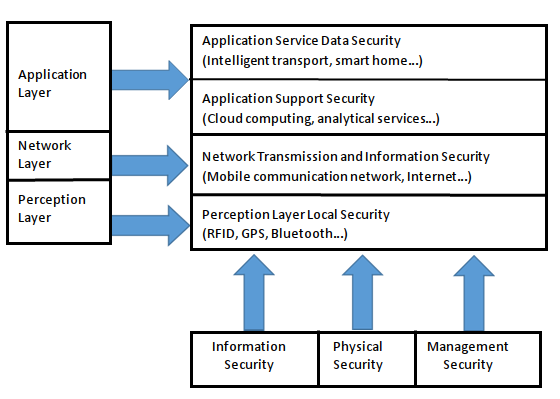
\includegraphics[width=\linewidth,height=10cm,keepaspectratio]{figure2_new.png}
	\caption{Internet of Things Architecture (adapted from \cite{Zhao6746513})}
	\label{fig:arch}
\end{figure}

\subsection*{Security Risks in the Perception Layer}
\addcontentsline{toc}{subsection}{Security Risks in the Perception Layer}
In the perception layer, devices are commonly found in public with minimal physical security. The literature states that there is a risk of an attacker physically
modifying a device at this layer. (\cite{Zhao6746513}; \cite{Xiaohui6643029}; \cite{Suo6188257}). Devices in the perception layer, for the most part,
are not very powerful. The devices use processors that prioritize efficiency and cost over speed. Due to this limitation, they are often unable to use the same security mechanisms found in traditional computers. 
(\cite{Suo6188257}; \cite{Granjal7005393}; \cite{Xiaohui6643029}). Even traditional attack methods used to target conventional computers could be 
used against the IoT. (\cite{Zhao6746513}). Attacks such as distributed denial of service (DDoS) could disrupt sensors from communicating with the devices that receive the gathered information. Devices in the perception layer are also suceptible to malware, as shown by the recent Mirai
botnet which infected thousands of IoT devices. (\cite{Incapsula}). 

\subsection*{Security Risks in the Network Layer}
\addcontentsline{toc}{subsection}{Security Risks in the Network Layer}
Many of the security risks in the network layer are already well-known, because they also apply to traditional computing platforms. 
(\cite{Zhao6746513}; \cite{Xiaohui6643029}). According to Zhao and Ge, the security implementations found in the network layer are fairly complete, but
the risks should not be ignored. The most common threats found in the network layer include man-in-the-middle attacks, illegal access due to 
insufficient authentication measures, information eavesdropping, and many others. These types of attacks put the privacy of users at risk as most
information transmitted is from the physical world. 

\subsection*{Security Risks in the Application Layer}
\addcontentsline{toc}{subsection}{Security Risks in the Application Layer}
Like the network layer, many of the security risks present in the layer are also found on traditional computing platforms. The literature outlines
risks such as software vulnerabilities and insecure authentication methods. (\cite{Zhao6746513}; \cite{Suo6188257}). Just like with traditional
platforms, mistakes by programmers that introduce vulnerabilities like buffer overflow are still common with IoT software. For authentication,
the developers must ensure that users are only allowed to access data they need. IoT devices commonly collect sensitive information that could
violate the privacy of the public if it got into the wrong hands. (\cite{Zhang:2015:EST:2714576.2737091}). 

\section*{IoT Security Protocol Standardization}
\addcontentsline{toc}{section}{IoT Security Protocol Standardization}

This section will first outline the need for a standardized suite of protocols to ensure security for the IoT. It will then evaluate various protocols
that have been proposed and outline any debate found in the literature. The protocols that will be discussed include the Constrained Application
Protocol (CoAP), Datagram Transport Layer Security (DTLS), and the Host Identity Protocol (HIP). 

\subsection*{The Need for Standardization}
\addcontentsline{toc}{subsection}{The Need for Standardization}
Many of the protocols required to ensure security for the IoT already exist but most IoT devices are not powerful enough to use them. (\cite{Keoh6817545}; \cite{Granjal7005393}; \cite{Garcia-Morchon:2013:SII:2462096.2462117}). Currently, standardization efforts are underway by the
Institute for Electrical and Electronics Engineers (IEEE) and the Internet Engineering Task Force (IETF). One project by the IETF is the
Constrained Application Protocol (CoAP). CoAP is a protocol similar to HTTP that allows devices to make requests and receive responses. (\cite{Keoh6817545}). The most commonly used protocol used to secure CoAP is Datagram Transport Layer Security (DTLS). (\cite{Keoh6817545}; \cite{Garcia-Morchon:2013:SII:2462096.2462117}). 
Some literature proposes the use of the Host Identity Protocol (HIP) as an alternative to DTLS. (\cite{Hummen}; \cite{Garcia-Morchon:2013:SII:2462096.2462117};). The conflict in the literature on this issue alone shows the need for standardization. As pointed out by Koeh et. al, the reason for the success of the HyperText Transfer Protocol (HTTP) has been the completely standardized protocol suite. For the Internet
of Things to have a successful and secure future, the industry must agree on a standardized security suite.

\subsection*{The Constrained Application Protocol}
\addcontentsline{toc}{subsection}{The Constrained Application Protocol}
The IETF decided that a new protocol was necessary to allow devices with limited resources to communicate efficiently. A working group was formed which came up 
with the idea for the Constrained Application Protocol (CoAP). The protocol allows devices to send and receive messages
in a way similar to HTTP. (\cite{Keoh6817545}; \cite{Capossele}). A universal resource identifier (URI) is used to make requests to destination devices and to
receive responses. In the figure below, a basic CoAP request and response is displayed. The client makes a ``GET'' request to the server at the location identified by the URI. In the ``GET'' request, the client requests the contents of ``temp.'' The server acknowledges the request with an ``ACK'' and sends the requested content back to the client. 

\begin{figure}[H]
	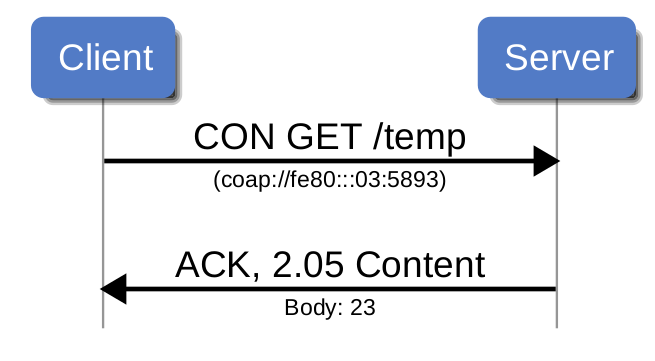
\includegraphics[width=\linewidth,height=5cm,keepaspectratio]{figure8.png}
	\caption{A Basic CoAP Interaction (\cite{Capossele})}
	\label{fig:arch}
\end{figure}

The major question currently in the literature is how this protocol should be secured. The subsections that follow will discuss various ways of securing
the Constrained Application Protocol. 

\subsection*{Datagram Transport Layer Security}
\addcontentsline{toc}{subsection}{Datagram Transport Layer Security}
This section will begin by discussing the findings of Garcia-Morchon et. al. regarding the viability of Datagram Transport Layer Security (DTLS)
for securing CoAP messages. To start with, DTLS is simply TLS over the UDP protocol instead of TCP. The CoAP recommends using DTLS in place of any
other method. The protocol is also considered to be the best suited protocol for securing CoAP messages. (\cite{Keoh6817545}). However, one major issue with DTLS is that it was designed for traditional networks. (\cite{Capossele}). 
The IETF has created a working group called ``DTLS In Constrained Environment'', whose goal is to 
come up with a DTLS implementation that is usable with the IoT. (\cite{Keoh6817545}). \\
~\newline
In a report by Garcia-Morchon et al., the authors analyzed the performance of DTLS using a custom application running on a Redbee Econotag. The device
was used to simulate a real world IoT device. The authors found that DTLS used a significant amount of memory due to the amount of messages sent. 
The authors also found that DTLS does not perform well in a network with high packet loss. \\
~\newline
The work of Garcia-Morchon et al. demonstrates the need for additional changes to enable DTLS to work with the IoT. 
Capossele, Cervo, De Cicco,
and Petrioli released a report outlining their optimized DTLS implementation. For their work, they used a MagoNode to simulate the presence of an
IoT device. The specifications of the test device were similar to the one used by Garcia-Morchon et al., but with 16 KB of RAM instead of 128 KB.
In order to make DTLS functional on their test device, the authors optimized modular arithmetic on large integers using their own assembly code.
The authors also created their own ECC library to further optimize the cryptographic functions. The authors analyzed the results by separating their
optimizations in order to see which ones had the greatest impact on performance. In the table below, one can see which optimization was performed,
the time the operation took, the energy used, and the increase in ROM usage. 

\begin{figure}[H]
	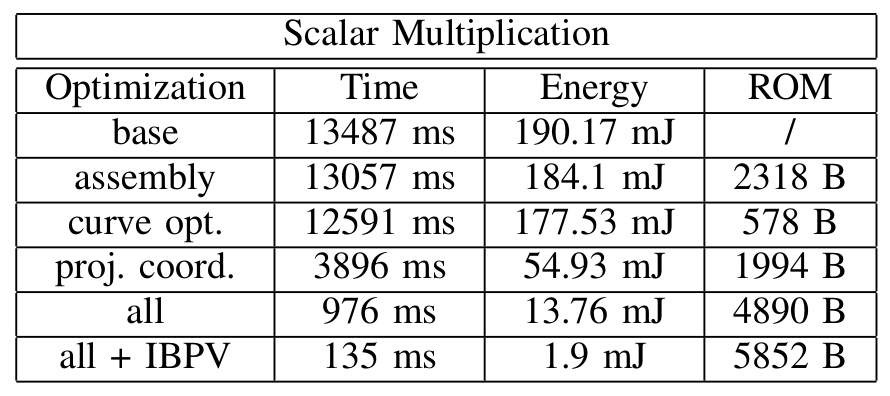
\includegraphics[width=\linewidth,height=5cm,keepaspectratio]{figure6.png}
	\caption{Scalar Multiplication Time Comparison (\cite{Capossele})}
	\label{fig:arch}
\end{figure}

As one can see from the figure, the optimizations together provide a large increase in performance when doing scalar multiplication, but at the expense of more ROM usage. 
The authors also analyzed how their optimizations improved the performance and energy usage when doing cyptographic functions. The figure below
shows their results. 

\begin{figure}[H]
	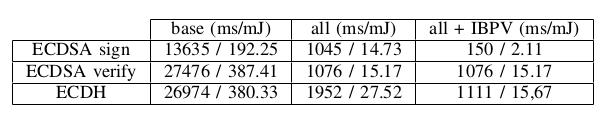
\includegraphics[width=\linewidth,height=7cm,keepaspectratio]{figure5.png}
	\caption{Overhead and Energy Consumption After Optimization (\cite{Capossele})}
	\label{fig:arch}
\end{figure}

Overall, the optimizations proposed by Capossele et. al. make DTLS a more viable option for securing the IoT.

\subsection*{Host Identity Protocol}
\addcontentsline{toc}{subsection}{Host Identity Protocol}

As mentioned in the previous section, DTLS is not extremely well suited for use with the IoT. An alternative
approach proposed by some literature is the use of the Host Identity Protocol (HIP). HIP makes use of public-key
cryptography to establish connections. (\cite{Hummen}; \cite{Garcia-Morchon:2013:SII:2462096.2462117}). However,
public-key cryptography is an expensive operation on a constrained platform like the IoT. Like DTLS, HIP must
be tailored for use with the IoT. This section will discuss two approaches proposed by the literature. 

\subsubsection*{HIP-DEX Optimizations proposed by Hummen et al.}
\addcontentsline{toc}{subsubsection}{HIP-DEX Optimizations proposed by Hummen et al.}
In an article by Hummen, Wirtz, Ziegeldorf, Hiller, and Wehrle, the authors analyzed the existing methods of 
implementing HIP and focused on HIP Diet EXchange (HIP DEX). The first major challenge the authors encountered
was the large amount of resources that public-key operations use. When an IoT device is performing a public-key operation,
it is often unable to do any of its other tasks. The expensive operations also make it possible for even a single attacker
to perform a denial of service attack on the device. In order to address these challenges, the authors proposed the following extensions to HIP DEX: 
a ``comprehensive session resumption mechanism'', a ``collaborative puzzle-based denial of service protection mechanism'', and a
``refined retransmission mechanism''. \\
~\newline
\textit{Session Resumption Mechanism}\\ 
~\newline
In the session resumption mechanism proposed by the authors, both devices will perform their most expensive protocol operations once during the handshake.
If the connection needs to be reestablished, the devices can used the information they have saved to securely resume the session using a lighter weight
session resumption handshake. The authors note that this technique could even be used with other protocols, such as DTLS. The technique does introduce some
security risks, however. Hummen et al. state that it is possible for an attacker who is eavesdropping on the communications to replay a saved resumption
handshake and gain unauthorized access to the network. In order to counteract this risk, a counter incremented upon each successful session resumption. 
When the authors evaluated the results of session resumption in isolation, they found that it reduced computational overhead by at least 85.7\%. \\
~\newline
\textit{DoS Protection Improvements}\\ 
~\newline
As mentioned previously, the authors proposed improvements to HIP DEX to reduce its vulnerability to denial of service (DoS) attacks. Currently to protect
from DoS attacks, HIP DEX requires a puzzle mechanism to be introduced when a DoS is detected by the device. During normal operation, the puzzle is not used.
Hummen et al. note that the mechanisms to detect an attack and to select an appropriate puzzle remain open research issues. In the authors proposal, attacks
would be detected by keeping track of the number of public-key operations performed within a specified period. If the limit is exceeded, then a puzzle will
be generated for the possible attacker. The authors propose that a high difficulty puzzle be generated for untrusted connections and a low difficulty puzzle
for trusted connections. When evaluating the results, the proposed DoS protection was found to successfully protect the IoT device from attack while still
allowing legitimate connections to take place. \\
~\newline
\textit{Retransmission Mechanism}\\ 
~\newline
The final extension proposed by the authors was a retransmission mechanism. Currently, the HIP DEX standard specifies an aggressive retransmission strategy
for handling the loss of messages. In their report, the authors propose an adaptive retransmission strategy that bases timeout values on the 
predicted transmission time for the message. However, it is possible that a device may have only received part of a message and a full retransmission
is not necessary. To address this, the authors propose the use of pre-fetching message information to delay the retransmission of messages while the 
remaining parts are still being transmitted. Finally, a new message type proposed by the authors allows the device responding to a message to notify the
sender that the message was received. This message would be send before the receiver does any cryptographic processing. When evaluating the results, 
Hummen et al. found that their retransmission strategy was a significant improvement over both HIP DEX and DTLS. The figure below shows their results.

\begin{figure}[H]
	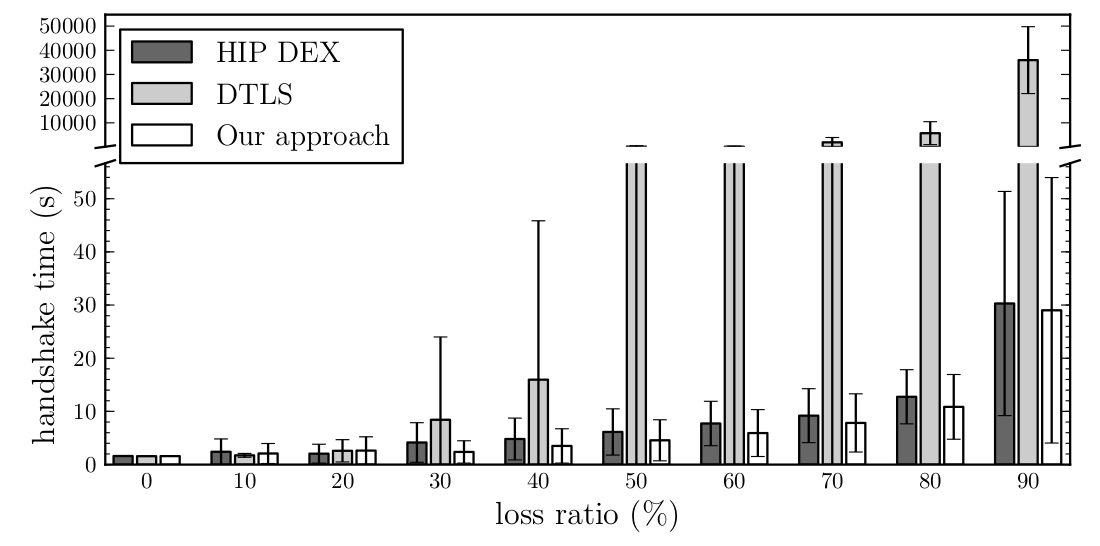
\includegraphics[width=\linewidth,height=6cm,keepaspectratio]{figure7.png}
	\caption{Results of HIP DEX Retransmission Strategy Optimization (\cite{Hummen})}
	\label{fig:arch}
\end{figure}

Overall, the extensions proposed by Hummen et al. provide a significant increase in performance for HIP DEX for use on constrained platforms like the 
IoT. However, there are also other approaches being considered by the literature. To conclude this section, the work of Garcia-Morchon, Keoh, Kumar,
Moreno-Sanchez, Vidal-Meca, and Ziegeldorf will be discussed. 

\subsubsection*{HIP-PSK proposition by Garcia-Morchon et al.}
\addcontentsline{toc}{subsubsection}{HIP-PSK proposition by Garcia-Morchon et al.}
In their report, the authors proposed an alternative version of HIP that they called HIP-PSK. Instead of using public-key cryptography, the authors chose
to use a pre-shared key (PSK). In their protocol, a more lightweight challenge-based authentication mechanism can be used instead of Diffie-Hellman key
exchange. The remainder of the protocol is identical to HIP-DEX. Garcia-Morchon et al. also propose the use of AMIKEY for key management with HIP-PSK
and their optimized DTLS implementation. To evaluate the results, the authors compared HIP-PSK to their own optimized version of DTLS. They found that 
HIP-PSK performed better than DTLS, but DTLS provided better interoperability. The authors did not compare HIP-PSK to HIP-DEX or any other variations. 

\section*{Government Action on IoT Security}
\addcontentsline{toc}{section}{Government Action on IoT Security}

This section will first begin by briefly discussing the current government regulations that can be found for Internet of Things devices. After that,
the section will discuss future standards and regulations that are being considered. This section will only focus on action from the U.S. government and the European Union.

\subsection*{Current Regulatory Environment}
\addcontentsline{toc}{subsection}{Current Regulatory Environment}

Currently, there are not many regulations or standards governing the manufacturing of IoT devices in both the U.S. and the EU. (\cite{Weber201023}; \cite{housecyberattacks}).  As discussed earlier in the report, there are standards that can help to ensure the security of IoT devices, but manufacturers are
not required to follow the standards. In a 2010 report by Weber, some requirements for future legislation are discussed. One of the most important 
requirements mentioned is that future legislation should be somewhat standardized around the world. Since businesses today do business all over the world,
it is important that they do not have to create separate versions of their devices for sale in countries with different regulations. During a hearing of the
U.S. House Energy and Commerce Committee, Representative Walden noted that one of the committee's goals was to make sure that new regulations on the IoT do not hinder innovation in the industry. 

\subsection*{Regulatory Proposals}
\addcontentsline{toc}{subsection}{Regulatory Proposals}

In the U.S. the Federal Trade Commission released a report analyzing the current state of the Internet of Things industry and released their recommendations
to Congress. This report will be discussed first, and after that, the proposals from the European Union will be discussed.

\subsubsection*{Federal Trade Commission Report}
\addcontentsline{toc}{subsubsection}{Federal Trade Commission Report}

\subsubsection*{European Union Proposals}
\addcontentsline{toc}{subsubsection}{European Union Proposals}

\section*{Conclusion}
\addcontentsline{toc}{section}{Conclusion}

The main purpose of this paper was to review the literature surrounding the security of the Internet of Things with a focus on the current security risks,
standards, and government regulations. As outlined in the report, the Internet of Things is a growing industry with lots of potential for innovation. 
However, the industry currently faces many security risks that have already resulted in the disruption of service on many websites. While the literature
seems to be in agreement on what the current risks are, there is some debate as to what kind of new standards should be used to mitigate them. Organizations
such as the IEEE have been working to come up with new standards that manufacturers can apply to their devices. One of the major challenges these researchers
will face is making these standards optimized enough to run on constrained platforms like the IoT. This is a major topic in the literature, with two major 
protocols that are being considered for use: Datagram Transport Layer Security and the Host Identity Protocol. While either of these standards would provide
adequate security for the IoT, manufacturers are not currently required to use either of them. The industry is currently self-regulating. Many governments
are considering the legislative options, but a major concern from U.S. lawmakers in particular is that more regulation will stifle innovation in the industry. 
Lawmakers in the European Union have been more aggressive, proposing a labeling requirement for IoT devices. Overall, researchers and lawmakers will need to
work together in order to come up with new ideas for securing the IoT. It is very likely that more security incidents will occur if manufacturers continue
to release devices with the security risks mentioned in this report. 
\newpage
\addcontentsline{toc}{section}{References}
\printbibliography
\end{flushleft}
\end{document}
